\section{LineObject}\label{lineObject}

Accepts NoteProcessors: no

Line Object

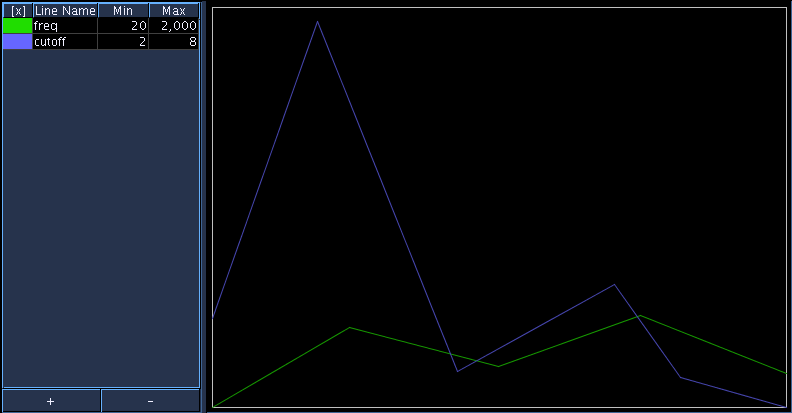
\includegraphics{images/lineObject.png}

Add and graphically edit global k-rate signals.

Use the bottom + and - buttons to add/remove lines.

Use the table to select a line. After selecting a line, you can edit the
points by dragging them, add points by clicking where you want the new
point, and remove points by rt-clicking them.

Use the table to edit the name of the signal, as well as the max and min
values (need to be floating point values). For editing the color of the
line, double-click the color box to the left of the lineName. A color
selection dialog will appear for the user to choose their desired color.

The name of the signal will be prepended with "gk" when outputing a
signal, i.e. a line name of "cutoff" will become "gkcutoff".
